\documentclass{beamer}
\usepackage[utf8]{inputenc}
\usepackage[T1]{fontenc}
\usepackage[francais]{babel}
\usepackage{graphicx}
\newtheorem*{theo}{Théorème} %%%%% ajout

\title[Introduction à la méthode de Monte-Carlo]{Résolution de l'équation de \textsc{Laplace}}
\subtitle{Introduction à la méthode de Monte-Carlo}
\author{Victor \textsc{Schneider}, Christophe \textsc{Riviere}, Fabien \textsc{Delhomme}}
\institute{UFR de mathématiques de Strasbourg}
\usetheme{Rochester}

\AtBeginSection[]
{
  \begin{frame}
    \frametitle{Table des matières}
    \tableofcontents[currentsection]
  \end{frame}
}
\setbeamertemplate{blocks}[rounded][shadow=true]

\begin{document}

\begin{frame}
    \titlepage
\end{frame}

\section{Introduction à la méthode de Monte-Carlo}

\begin{frame}{Qu'est-ce qu'est cette méthode ?}
    \begin{itemize}
        \item La méthode de Monte-Carlo est une méthode d'approximation de
            résultat numérique par l'usage de probabilités.
        \item Son invention fut révolutionnaire de par l'approche qu'elle envisageait :
            \begin{itemize}
                \item On utilise en général des données statistiques pour en
                    déduire des probabilités.
                \item La méthode de Monte-Carlo, elle, déduit les solutions d'un
                    problème déterministe à partir des probabilités !
            \end{itemize}
    \end{itemize}
\end{frame}


\begin{frame}{L'origine de cette méthode}
    \begin{itemize}
        \item Elle fut inventée en 1946 par \emph{Stanislaw Ulam}, physicien
            américain qui travaillait sur le projet Manhattan, et  \emph{John
            von Neumann}, mathématicien, américain également.
        \pause
        \medbreak
        \item Le projet étant top secret, il avait besoin d'un nom de code.
            L'équipe scientifique décida alors de lui donner le nom de
            \emph{Monte-Carlo}, en référence au casino du même nom à Monaco.
    \end{itemize}
\end{frame}


\begin{frame}{Utilisation actuelle}
    C'est une méthode fréquemment employé de nos jours dans les laboratoires
    pour déterminer des solutions numériques à partir des modèles théoriques,
    car :
    \begin{itemize}
        \item elle donne des résultats d'une bonne précision.
        \item la puissance des ordinateurs actuelle est largement suffisante
            pour pouvoir générer beaucoup de nombres pseudo aléatoires en un
            temps réduit.
    \end{itemize}
    Elle est aussi employée dans la finance (ex : calculs de risque ) et bien
    d'autres domaines, car elle donne des prédictions en général plus précise
    que les autres méthodes d'analyse.
\end{frame}

\section{Présentation théorique de la méthode de Monte-Carlo}

\begin{frame}{Idées cachées derrière cette méthode}
    Derrière cette méthode se cachent deux théorèmes majeurs.
    \medbreak
    Le premier nous dit que l'on peut peut voir les grandeurs (d'une certaine forme) comme des espérances. C'est le \alert{Théorème de Transfert}.
\end{frame}

\begin{frame}{Idées cachées derrière cette méthode}
    \begin{theo}
        Théorème de transfert dans le cas d'une loi continue.

        Soit $f : \mathbb{R}^n \rightarrow \mathbb{R}$ la fonction densité associée à la variable
        aléatoire $X = (X_1, X_2,...,X_n)$.

        Alors\[ \mathbb{E} \left( \phi(X_1, ..., X_n) \right) =  \int_{\mathbb{R}^n}
        \phi(x_1,...,x_n)f(x_1,...,x_n) \, \mathrm{d}x_1...\mathrm{d}x_n.  \] 
    \end{theo}
\end{frame}

\begin{frame}{Idées cachées derrière cette méthode}
    Le second théorème nous dit que si l'on a l'espérance d'une variable
    aléatoire $X$, alors on peut approcher cette espérance en faisant beaucoup
    de fois l'expérience donnant $X$, et en prenant la moyenne des résultats
    obtenus. Autrement dit l'espérance est l'équivalent probabiliste, lorsque
    l'on a un grand nombre d'expérience, de la moyenne statistique. C'est la
    \alert{Loi des Grands Nombres}.
\end{frame}

\begin{frame}{Idées cachées derrière cette méthode}
    \begin{theo}
     Loi forte des grands nombres.

    Soit $(X_k)_{k\ge 0}$ une suite de variables aléatoires indépendantes et suivant toutes la même loi, à valeurs dans $\mathbb{R}^n$. On suppose $\mathbb{E}(|X_1|) < +\infty $. Alors
    \[
        \frac{X_1+...+X_N}{N}\underset{N\to+\infty}{\longrightarrow}\mathbb{E}(X_1)\; \text{presque sûrement.}
    \]
\end{theo}
\end{frame}

\begin{frame}{Idées cachées derrière cette méthode}
    En combinant ces deux théorèmes, on peut alors donner une estimation de notre valeur numérique, que l'on aura exprimée comme une espérance.
    \smallbreak
    Cette estimation dépend bien sur du nombre de d'expériences que l'on simulera.
    \smallbreak
    Ces deux théorèmes justifient donc l'existence de cette méthode.
\end{frame}

\begin{frame}{Le problème de Dirichlet discret}
    On cherche à résoudre ce problème, appelé \emph{Problème de Dirichlet}, en utilisant la méthode de Monte-Carlo :
    \smallbreak
    Soit $\Omega \in \mathbb{R}$ un domaine borné, et $\partial\Omega$ son bord. On cherche $u$ telle que
\[\bigtriangleup u(x) = 0, \quad \forall x \in \Omega\]
\[u(x) = g(x), \quad \forall x \in \partial \Omega, \quad \text{g connue}\]
\end{frame}

\begin{frame}{Le problème de Dirichlet discret}
    Premier problème qui se présente : les ordinateurs ne gèrent pas la notion
    de \emph{continuité}. Il va donc falloir \emph{discrétiser} tout ça.
\end{frame}


\begin{frame}{Le problème de Dirichlet discret}
    La résolution technique de cette discrétisation sera vue plus tard, mais
    avant ça expliquons pourquoi le problème de Dirichlet et sa contre-partie
    le problème de Dirichlet discret sont équivalents (ou au moins asymptotes)
    lorsque l'on prend un pas suffisamment petit.
\end{frame}


\begin{frame}{Le problème de Dirichlet discret}
    \begin{figure}[htp]
        \centering
        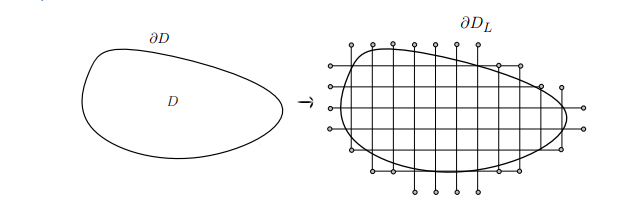
\includegraphics[width=4cm]{domainediscret}
        \caption{Discrétisation d'un domaine quelconque dans $\mathbb{R}^2$}
        \label{Domaine discret}
    \end{figure}
\end{frame}


\begin{frame}{Le problème de Dirichlet discret}
    Appelons $h$ notre pas. On comprend que si $(x,y)$ est dans une "case",
    alors $(x+h, y)$ sera dans la case à sa droite, $(x-h, y)$ sera dans celle
    à sa gauche, etc.  \medbreak

    \begin{block}{Définition}
        On va montrer que $\bigtriangleup u$ peut
        alors être approché par le \emph{Laplacien Discret}, défini par :
        \[
            \overline{\bigtriangleup}F = \sum\limits_{\substack{\Omega_d \cup \partial \Omega_d \\ y \sim x}} (F(y) - F(x))
        \]
        avec $y\sim x$ signifiant que $y$ est voisin de $x$ et $\Omega_d$ le domaine discrétisé.
    \end{block}

\end{frame}


\begin{frame}{Le problème de Dirichlet discret}
    $u$ prend ses valeurs dans $\mathbb{R}^2$, la formule de Taylor nous donne
    (on travaille sur les abscisses mais c'est exactement pareil pour les
    ordonnées) :
    \[
        \begin{cases}
            u(x+h,y) - u(x,y) &=  h\partial_1 u(x,y) + \frac{h^2}{2}\partial_1^2 u(x,y)+ O(h^3)\\
            u(x-h,y) - u(x,y) &=  -h\partial_1 u(x,y) + \frac{h^2}{2}\partial_1^2 u(x,y)+ O(h^3)\\
        \end{cases}
    \]
    \begin{block}{En sommant les deux on obtient:}

        \begin{eqnarray*}
            \partial_1^2 u(x,y)&=& \frac{\left[(u(x+h,y) - u(x,y)) + (u(x-h,y) - u(x,y)) \right]}{h^2} \\
            & & + O(h)
        \end{eqnarray*}
    \end{block}

\end{frame}

\begin{frame}{Le problème de Dirichlet discret}
    On a alors
    \[
    \bigtriangleup F = \frac{1}{h^2}\overline{\bigtriangleup}F + O(h)
    \]
    avec $\overline{\bigtriangleup}$ le laplacien discret.On peut donc
    approcher le problème de Dirichlet par celui suivant, appelé problème de
    Dirichlet discret :
    \[\overline{\bigtriangleup} u(x) = 0, \quad \forall x \in \Omega_d\]
    \[u(x) = g(x), \quad \forall x \in \partial \Omega_d, \quad \text{g connue}\]
\end{frame}


\begin{frame}{Résolution du problème de Dirichlet discret}
    \begin{block}{Résultats admis}
        Nous ne le montrerons pas, mais il a été démontré que dans le cas d'une
        marche aléatoire, au bout d'un certain temps on peut atteindre n'importe
        quel point de l'espace. Autrement dit, dans la marche de l'ivrogne,
        l'ivrogne finit toujours par rentrer chez lui !
    \end{block}

    \pause

    \begin{block}{Résultats admis}
        De même, si l'on part de n'importe quel point de notre espace discrétisé,
        avec une marche aléatoire on atteindra forcément un point du bord de
        l'espace.
    \end{block}

\end{frame}

\begin{frame}{Résolution du problème de Dirichlet discret}
    Intervient alors notre dernier théorème :

    \begin{theo}
     $\forall x \in \Omega_d$, la valeur de $u(x)$ est donnée par :
     \[
        u(x) = \sum_{y\in \partial \Omega_d} g(y) P(x, \{y\})
     \]
     avec $P(x, \{y\})$ la probabilité que $y$ soit le premier élément de $\partial \Omega_d$ atteint par la marche aléatoire partant de $x$.
\end{theo}
\end{frame}

\begin{frame}{Résolution du problème de Dirichlet discret}
    Ce théorème donne alors directement la méthode nécessaire pour programmer
    de quoi résoudre le problème de Dirichlet discret numériquement en tout
    point $x$ de l'espace discrétisé. En effet :
    \begin{itemize}
        \item $g$ est connue, car c'est une donnée du problème
        \pause
        \item On peut également déterminer quels sont les points en bordures de notre espace
        \pause
        \item Pour approcher $P(x,{y})$, il suffit de simuler un grand nombre
            de fois l'évènement et de faire la moyenne des résultats obtenus.
    \end{itemize}
    Attelons-nous y dès maintenant !
\end{frame}

\section[Implémentation du schéma numérique]{Implémentation de la méthode de Monte-Carlo}

\begin{frame}{Le principe de la méthode de Monte-Carlo}
    Nous avons choisi de représenter notre domaine par une matrice de $0$ et de $1$, pour représenter un domaine de ce type :
    \begin{figure}[htp]
        \centering
        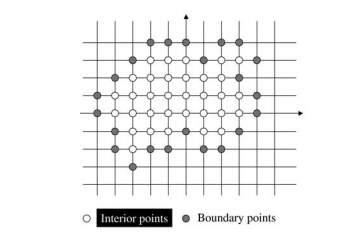
\includegraphics[width=4cm]{domainediscretmatrice}
        \caption{Discrétisation d'un domaine quelconque dans $\mathbb{R}^2$}
        \label{Domaine discret}
    \end{figure}
    \pause
    \begin{itemize}
        \item Un domaine discrétisé
        \pause
        \item Une fonction définie sur le bord discrétisé du domaine
    \end{itemize}
\end{frame}

\begin{frame}{La marche aléatoire}
    \begin{itemize}
        \item À partir de chaque point du domaine, on réalise des marches
            aléatoires, toutes partant de ce point.
        \pause
        \item À chaque réalisation correspond une valeur trouvées au bord
        \pause
        \item On fait la moyenne des valeurs obtenues
    \end{itemize}
\end{frame}

\section{La valeur trouvée approxime-t-elle la solution de l'équation ?}

\subsection{Écriture du code, les choix que nous avons faits}

\begin{frame}{Un enjeu majeur}
    \begin{alertblock}{Enjeu majeur}
        \Large{Comment représenter numériquement les éléments du problème ?}
    \end{alertblock}
\end{frame}

\begin{frame}{Représentation du domaine}
    \begin{block}{Définition}
        On définit $N$ tel que $\frac{1}{N}$ soit de pas du maillage. \\
        Ainsi plus $N$ est grand, plus on se rapproche du domaine continu réel.
    \end{block}
\end{frame}

\begin{frame}{Représentation du domaine}
    \begin{alertblock}{Un mauvais choix}
        Représenter le domaine par sa fonction indicatrice
    \end{alertblock}
    \begin{block}{Un meilleur choix}
        Créer une matrice pour représenter le domaine
    \end{block}
\end{frame}
\begin{frame}
    Par exemple, pour $N=11$:
    \[ \left(\begin{array}{ccccccccccc}
            0& 0& 0& 0& 0& 0& 0& 0& 0& 0& 0\\
            0& 0& 0& 0& 1& 1& 0& 0& 0& 0& 0\\
            0& 0& 0& 1& 1& 1& 1& 0& 0& 0& 0\\
            0& 0& 1& 1& 1& 1& 1& 1& 0& 0& 0\\
            0& 0& 1& 1& 1& 1& 1& 1& 1& 0& 0\\
            0& 0& 1& 1& 1& 1& 1& 1& 1& 0& 0\\
            0& 0& 0& 1& 1& 1& 1& 1& 0& 0& 0\\
            0& 0& 0& 0& 1& 1& 1& 0& 0& 0& 0\\
            0& 0& 0& 0& 0& 0& 0& 0& 0& 0& 0
        \end{array}\right)
    \]
\end{frame}

\begin{frame}{Autre éléments du programme}
    \begin{itemize}
        \item La fonction définie au bord du domaine,
        \item La réalisation de la marche aléatoire à partir d'un point,
        \item Le nombre $K$ de marches aléatoires pour chaque point. Plus il est grand, plus on 
            se rapproche de la solution.
        \item Une procédure qui calcule les valeurs de la solutions; ces dernière sont placées dans une matrice représentent la discrétisation de la solution.
    \end{itemize}
\end{frame}

\section{Présentation du programme final}

\section{Convergence de la méthode de Monte-Carlo}

\begin{frame}{Rappels des définitions}
    \begin{block}{On rappel que l'on a choisit pour plus de commodité}
        \begin{itemize}
            \item De se placer dans un domaine compris dans le pavé $[0;1]^2$,
            \item On note $N$ le paramètre de discrétisation du domaine,
            \item On note $K$ le nombre de marche aléatoire lancée par point,
                (On aura donc lancé à la fin de l'algorithme $K*N^2$ marches aléatoires)
            \item On note $\partial \Omega$ le bord du domaine $\Omega$,
            \item On note $M$ la matrice qui représente la solution approchée:
                $\forall i,j \in [1;N] \quad M(i,j) = f(\frac{x}{N}, \frac{y}{N})$
        \end{itemize}
    \end{block}
\end{frame}

\begin{frame}{Choix pour calculer la convergence}
    Afin de déterminer l'ordre de convergence de la méthode de Monte-Carlo, nous avons choisi une
    solution évidente de l'équation de \textsc{Laplace}. En effet, soit
    \[
        f(x,y) = a*x + b*y + c \quad \mbox{ Où } a, b \in \mathbb{R}
    \]
    Alors nous avons trivialement:
    \[
        \frac{\partial^2 f}{\partial x^2} + \frac{\partial^2 f}{\partial y^2} = 0
        \qquad \mbox{Et, } \forall x,y \in \partial \Omega \quad f(x,y) = g(x,y)
    \]
    \begin{block}{On a donc}
        $f(x,y) = a*x + b*y + c$ qui est solution du problème de \textsc{Dirichlet} avec la condition au bord $g(x,y) = f(x,y)$.
    \end{block}

\end{frame}

\begin{frame}{Choix de la norme}
    \begin{block}{Norme infinie}
        On peut donc calculer la distance entre notre solution partielle donnée par la matrice $M$
        et la solution exacte, en fonction de $K$ et de $N$:
        \[
            e_{K, N} = \sup_{i,j \in [1;N]}{| M(i/N,j/N) - g(x,y)|}
        \]
    \end{block}
\end{frame}

\begin{frame}{Astuce pour calculer la convergence}
    \begin{block}{Problème:}
        Il s'avère que le programme pour $K \approx 50$ et $N\approx 30$ est assez long à exécuter.
        Or on veut lancer le programme pour plusieurs $K$ pour un $N$ fixé.
    \end{block}

    \begin{alertblock}{Question:}
        \centering \huge{Comment faire ?}
    \end{alertblock}
\end{frame}

\begin{frame}{Solution}
    \begin{block}{Il s'avère...}
        ... Que l'on peut fusionner deux schémas qui ont le même $N$ !
    \end{block}
    \begin{block}{Explication}
        Soit deux matrices représentants respectivement la solution approchée pour $N$ fixée, et avec le nombre de marche aléatoire de $K$ et $l$.
        Alors, on peut calculer la matrice qui est une représente de la solution approchée avec comme paramètre $N$ et $K+l$ !
    \end{block}
\end{frame}

\begin{frame}{Application}
    Nous avons donc afficher la distance entre la solution approchée et la solution finale pour 
    $K$ qui variaient avec la formule de la moyenne pondérée:

    \[
        M_{K+l}(i,j) = \frac{ \sum_{i=K}^{i=K+l} v_i + K*M_{K}(i,j) }{ (K + l) }
    \]
\end{frame}

\begin{frame}{Résultat}
    \begin{figure}
        \centering 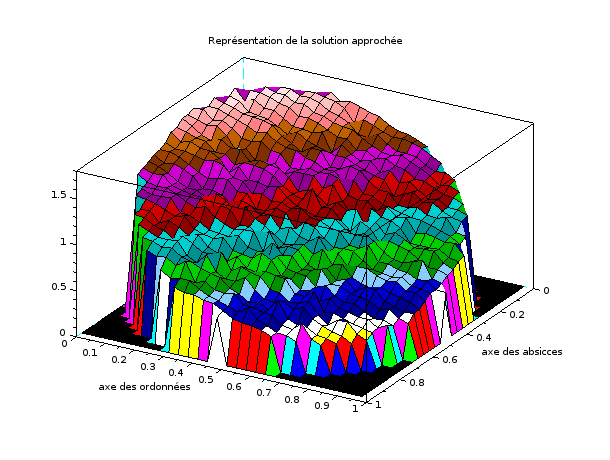
\includegraphics[width=10cm]{ResultatsConvergences/ImageK5S25N30.png}
    \end{figure}
\end{frame}

\begin{frame}{Résultat}
    \begin{figure}
        \centering 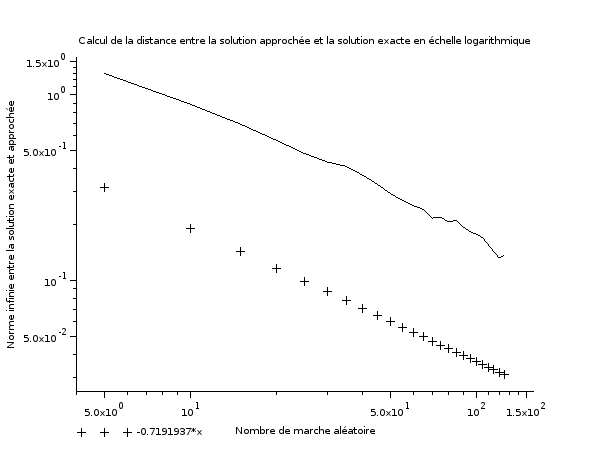
\includegraphics[width=10cm]{ResultatsConvergences/Convergence_K5_S25_N30.png}
    \end{figure}
\end{frame}

\section{Conclusion}

\begin{frame}
    On distingue quelques avantages de la méthode de Monte-Carlo par rapport aux méthodes plus classiques...
    \pause
    \begin{itemize}
        \item L'implémentation du schéma est plutôt simple (!)
        \pause
        \item La solution est calculée point par point.
    \end{itemize}
\end{frame}

\begin{frame}
    Qui s'accompagne de quelques inconvénients :
    \pause
    \begin{itemize}
        \item Convergence \alert{faible} (On a trouvé en moyenne une convergence de l'ordre de $O(\frac{1}{K^{0.67}}$)
        \pause
        \item Dépend de la «qualité» du hasard que l'on utilise pour la marche aléatoire.
        \pause
        \item Difficulté théoriques pour prouver la convergence pour tout domaine donné.
        \pause
        \item Il est aussi très difficile d'améliorer l'ordre de convergence de cette méthode.
    \end{itemize}
\end{frame}

\end{document}
